%%%%%%%%%%%%%%%%%%%%%%%%%%%%%%%%%%%%%%%%%%%%%%%
%
% Template for Bachelor degrees
% DISI - Dipartimento di Ingegneria e Scienza dell’Informazione
% DISI - Department of Information Engineering and Computer Science
%
% update 2020-08-30
%
% To generate pdf 
% pdflatex __filename__.tex
% bibtex __file_name__.aux
% pdflatex __file_name__.tex
% pdflatex __file_name__.tex
%
%%%%%%%%%%%%%%%%%%%%%%%%%%%%%%%%%%%%%%%%%%%%%%%

% 2 side format
\documentclass[epsfig,a4paper,11pt,titlepage,twoside,openany]{book}
\usepackage{epsfig}
\usepackage{plain}
\usepackage{setspace}
\usepackage[paperheight=29.7cm,paperwidth=21cm,outer=1.5cm,inner=2.5cm,top=2cm,bottom=2cm]{geometry} % layout setting
\usepackage{titlesec} % custom setup title of chanpter
% \usepackage{newtxtext,newtxmath} % times new roman

%%%%%%%%%%%%%%
% support for accented letters
%
%\usepackage[latin1]{inputenc} % Windows;
\usepackage[utf8x]{inputenc} % Linux (unicode package is required);
%\usepackage[applemac]{inputenc} % Mac.

\singlespacing

% italian language
%\usepackage[italian]{babel}

\begin{document}

  % no page number
  \pagenumbering{gobble} 
  \pagestyle{plain}

\thispagestyle{empty}

\begin{center}
  \begin{figure}[h!]
    \centerline{
\psfig{file=marchio_unitrento_colore_it_202002.eps,width=0.6\textwidth}}
  \end{figure}

  \vspace{2 cm} 

  \LARGE{Department of Information Engineering and Computer Science\\}

  \vspace{1 cm} 
  \Large{Bachelor's Degree in\\
    
    % Computer Science
    Computer, Communication and Electronic Engineering
    % Information and Communications Engineering
    % Information and Business Organization Engineering
    % Electornics and Telecommunications Engineerign
  }

  \vspace{2 cm} 
  \Large\textsc{Final Dissertation\\} 
  \vspace{1 cm} 
  \Huge\textsc{Title\\}
  \Large{\it{Sub-title (optional)}}


  \vspace{2 cm} 
  \begin{tabular*}{\textwidth}{ c @{\extracolsep{\fill}} c }
  \Large{Supervisor} & \Large{Student}\\
  \Large{Alberto Montresor}& \Large{Marco Morandin}\\
  \end{tabular*}

  \vspace{2 cm} 

  \Large{Academic year 2023/2024}
  
\end{center}



  \clearpage
 
%%%%%%%%%%%%%%%%%%%%%%%%%%%%%%%%%%%%%%%%%%%%%%%%%%%%%%%%%%%%%%%%%%%%%%%%%%
%%%%%%%%%%%%%%%%%%%%%%%%%%%%%%%%%%%%%%%%%%%%%%%%%%%%%%%%%%%%%%%%%%%%%%%%%%
%% Note
%%%%%%%%%%%%%%%%%%%%%%%%%%%%%%%%%%%%%%%%%%%%%%%%%%%%%%%%%%%%%%%%%%%%%%%%%%
%% Thanks/ Acknowledgements section is optional
%%%%%%%%%%%%%%%%%%%%%%%%%%%%%%%%%%%%%%%%%%%%%%%%%%%%%%%%%%%%%%%%%%%%%%%%%%
%%%%%%%%%%%%%%%%%%%%%%%%%%%%%%%%%%%%%%%%%%%%%%%%%%%%%%%%%%%%%%%%%%%%%%%%%%
  \thispagestyle{empty}

\begin{center}
  {\bf \Huge Acknowledgements}
\end{center}

\vspace{4cm}


\emph{
  ...thanks to...
}

  \clearpage
  \pagestyle{plain} % no heading, footer with centered page number

  
  % page number with Arabic format
  \mainmatter

%%%%%%%%%%%%%%%%%%%%%%%%%%%%%%%%%%%%%%%%%%%%%%%%%%%%%%%%%%%%%%%%%%%%%%%%%%
%%%%%%%%%%%%%%%%%%%%%%%%%%%%%%%%%%%%%%%%%%%%%%%%%%%%%%%%%%%%%%%%%%%%%%%%%%
%% Note
%%%%%%%%%%%%%%%%%%%%%%%%%%%%%%%%%%%%%%%%%%%%%%%%%%%%%%%%%%%%%%%%%%%%%%%%%%
%% The maximum number of pages is 30, including:
%%   index
%%   abstract
%%   chapters
%% Excluding:
%%   frontispiece
%%   acknowledgements 
%%   attachments
%%
%% For further details and updated rules, please check the guidelines.
%%%%%%%%%%%%%%%%%%%%%%%%%%%%%%%%%%%%%%%%%%%%%%%%%%%%%%%%%%%%%%%%%%%%%%%%%%
%%%%%%%%%%%%%%%%%%%%%%%%%%%%%%%%%%%%%%%%%%%%%%%%%%%%%%%%%%%%%%%%%%%%%%%%%%

    % index
    \tableofcontents
    \clearpage
    
    
          
    % group to define space between chapters
    \begingroup
      % no page break between chapters
      % override clear page commands
      \renewcommand{\cleardoublepage}{} 
      \renewcommand{\clearpage}{} 
      % override format of title chapter
      % from
      %   Chapter X
      %   Title
      % to
      %   X   Title
      
      \titleformat{\chapter}
        {\normalfont\Huge\bfseries}{\thechapter}{1em}{}
        
      \titlespacing*{\chapter}{0pt}{0.59in}{0.02in}
      \titlespacing*{\section}{0pt}{0.20in}{0.02in}
      \titlespacing*{\subsection}{0pt}{0.10in}{0.02in}
      
      % summary / abstract
      \chapter*{Abstract} % no number
\label{abtract}

\addcontentsline{toc}{chapter}{Abstract} % add to index







%%%%%%%%%%%%%%%%%%%%%%%%%%%%%%%%%%%%%%%%%%%%%%%%%%%%%%%%%%%%%%%%%%%%%%%%%%
%%%%%%%%%%%%%%%%%%%%%%%%%%%%%%%%%%%%%%%%%%%%%%%%%%%%%%%%%%%%%%%%%%%%%%%%%%
%% Note
%%%%%%%%%%%%%%%%%%%%%%%%%%%%%%%%%%%%%%%%%%%%%%%%%%%%%%%%%%%%%%%%%%%%%%%%%%
%% The abstract is a short summary of the work describing the target,
%% the subject of the thesis, the methodology and the techniques,
%% the data collection and elaboration, the explanation of the
%% reached results and the conclusion.
%% The abstract of the dissertation must have a maximum length of 3 pages
%% and must include the following information:
%%   context and motivation
%%   short summary of the main problem you have dealt with
%%   developed and /or used techniques 
%%   reached results, the personal contribution of the student has to be highlighted
%%%%%%%%%%%%%%%%%%%%%%%%%%%%%%%%%%%%%%%%%%%%%%%%%%%%%%%%%%%%%%%%%%%%%%%%%%
%%%%%%%%%%%%%%%%%%%%%%%%%%%%%%%%%%%%%%%%%%%%%%%%%%%%%%%%%%%%%%%%%%%%%%%%%%      
      
      %%%%%%%%%%%%%%%%%%%%%%%%%%%%%%%%
      % chapters
      %
      % \input or \include
      %
        \chapter{Introduction}
\label{cha:789}

        \chapter{State of the art}
\label{cha:intro}
\section{Industrial IOT}
\section{Industry 4.0}
\subsection{Timeseries Data}
\subsection{Timeseries Database}
\section{Industry 5.0}
\subsection{Retrofitting legacy devices}
\subsection{Predictive maintenance}

        \chapter{Methodology}
\label{cha:789}
This chapter is about how the implementation of predictive maintenance of legacy devices is done in this dissertation. The data collection part of the project was done during my internship ad Thinkin, a software house situated in Trento.
\section{Problem Definition}
The goal is to retrofit legacy equipment that is working today but does not have support for sensor data collection due to lack of sensors or inability to access data, and add some data analytics such as predictive maintenance.
\section{Operational Framework}
In order to implement predictive maintenance, it was determined that a framework should be employed whereby external sensors are installed on a device and monitor its inputs and outputs. This allows for the understanding of whether the device in question requires maintenance or not.\\
	\begin{figure}[h!]
    \centerline{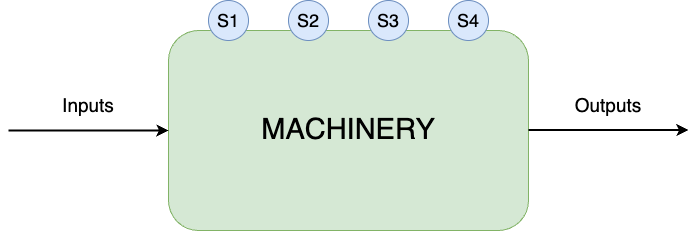
\psfig{file=operational_framework.png, width=0.7 \textwidth}}
  	\end{figure}
  	\\So the framework can be generalised as follows:
  	\[Remaining\ Useful\ Life\ =\ f(Input,\ Output, \overline{S}\ )\]
  	The framework presented above allows for the observation of input and output as well as sensor data, in order to identify a function that can approximate the remaining useful life of the equipment in question.
\section{Requirements}
Given the intended real-world context of this project, which involves multiple users, each with multiple machines and sensors that transmit data at regular intervals, it is essential to implement a robust software architecture capable of handling high throughput and a vast volume of data without compromising data integrity or introducing errors. Furthermore, the objective was to develop an architecture that could be readily scaled horizontally, allowing for the project's growth to be managed effectively. 
\subsection{Used Technology}
This section introduces the software technologies utilised in the project to fulfil the requirements of the preceding section. The objective is to underscore the decision to employ professional technologies that are readily scalable on a large scale, achieve optimal performance and are reliable. Additionally, they possess the benefit of being all open source technologies.
\subsubsection{MQTT}
MQTT is a publish-subscribe network protocol that is widely utilised in the field of Internet of Things due to its minimalistic design. It is an open OASIS standard and an ISO recommendation.\\
MQTT defines two actors in the network: a message broker, which receives all messages from clients and routes them to the appropriate destination clients; and clients, which are all devices that are connected to a message broker. The communications are structured into a hierarchical topic model, in which clients can publish or subscribe.\\
MQTT is designed to operate on constrained bandwidth and reliably transmit messages, even across unstable or high-latency networks. The protocol's keep-alive feature and minimal header size make it an optimal choice for IoT since it could be implemented in devices with microcontrollers. The lightweight nature of MQTT enables it to connect a considerable number of clients simultaneously to the same message broker.\\
\subsubsection{Kafka}

\subsubsection{Timescale DB}
Timescale is a time series database built on PostgreSQL, extending it with time-series optimisations. In comparison to PostgreSQL, Timescale offers a number of additional features, including automatic data partitioning, high ingest rates, and compression techniques optimised for time series data. The result is that queries on time series are thousands times faster in comparison with PostgreSQL. Due to the fact that timescale uses SQL with some additional function make it simpler to learn compared to other time series databases. Moreover, as an extension of PostgreSQL, it benefits from the reputation built up over twenty-five years of existence. This makes it an excellent choice, as it is a guarantee of a widely known, solid database management system. Furthermore, between versions, there are no radical changes that make the work already done inapplicable.
\section{Software Architecture and Implementation}
The software architecture designed to facilitate predictive maintenance of legacy machinery is structured with micro services to enable horizontal scalability and facilitate maintenance of the various software components.
\\The following image depicts the software architecture in use. Rectangles represent developed services, ovals represent used services, and the cylinder represents the database.
\begin{figure}[h!]
    	\centerline{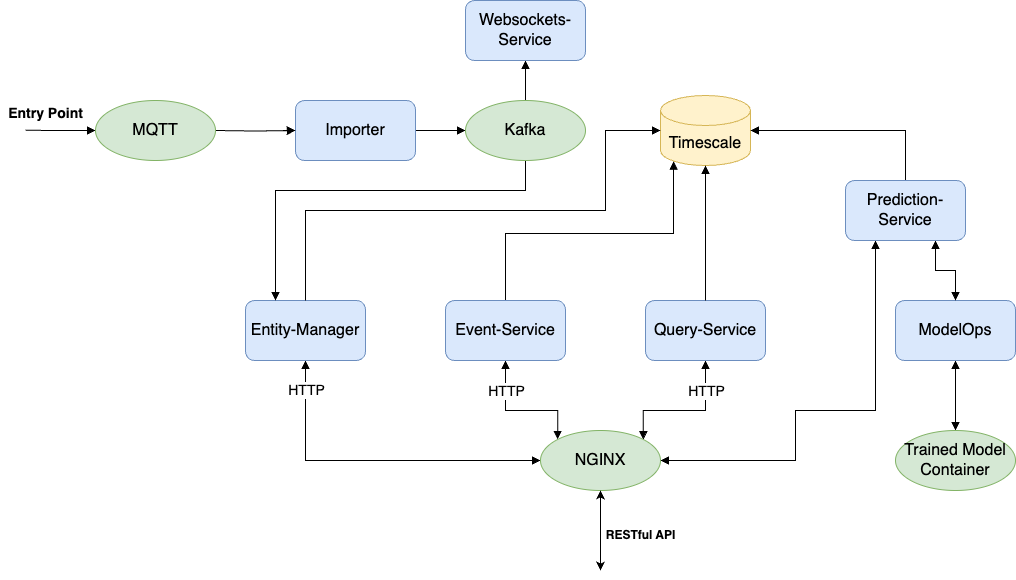
\psfig{file=architettura.png, width=1.1 \textwidth}}
\end{figure}
\\The data flow begins with MQTT, where data from all sensors registered in the system are published. From there, a micro service called "importer" is responsible for reading the data published on MQTT and publishing it to a topic on Kafka. The importer is a straightforward module that ensures optimal reliability and efficiency in data persistence. Subsequently, a micro-service designated as the "entity-manager" is responsible for database management and data storage from Kafka to Timescale. This service provides a suite of RESTful APIs that facilitate control over the entities stored in the database. In the system, data is divided into deployments, which represent the various clients. Deployments are divided into zones, which represent areas of a factory or locations. In the various zones, there are different assets, which represent machinery. Finally, each zone contains the various sensors installed. In the picture below you can see the ER schema of the database. It is intended to point out that the sensor-data and asset-status tables are Timescale hyper tables and are weak relationships, which means that the data are identified by the instant at which they were recorded and by the relationship they have to the other entity to which they are linked.
	\begin{figure}[h!]
    	\centerline{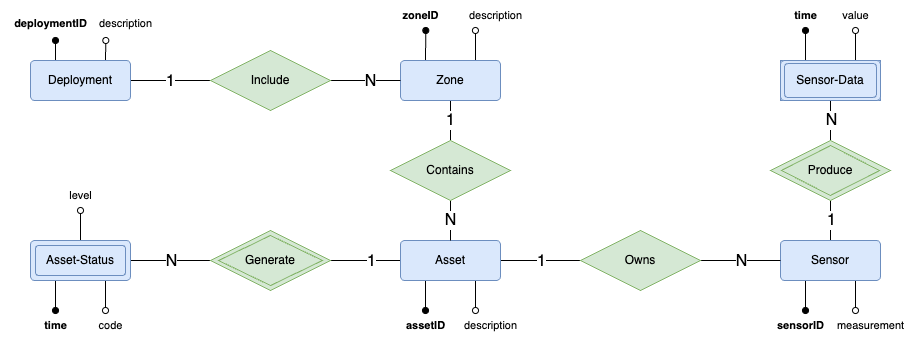
\psfig{file=schemaER.png, width=1.1 \textwidth}}
  	\end{figure}
 \\With the API, these entities can be created, deleted, and visualised. Additionally, for each asset, the status is saved in a dedicated table, representing any malfunctions encountered. Finally, a table containing the data of all sensors with a reference to the corresponding sensor is available. The "entity-manager" service is also responsible for reading data from Kafka and saving it to Timescale in such a way that it is saved persistently and efficiently. This is because complex queries can be made on Timescale and data compression is much more efficient. Furthermore, a service designated as the "query service" has been developed to facilitate the execution of queries on sensor data via RESTful APIs. This service aggregates the results into buckets of a size selected by the user. Additionally, an "event service" has been created to generate events on sensor data through the creation of RESTful API rules comprising mathematical formulas. The latter two services are beneficial for the generation of statistical data on the operation of a machine. Finally, with regard to predictive maintenance, a service called "prediction-service" has been created that, through an HTTP endpoint, provides the prediction of the remaining life of the machinery. This service takes care of making a query on Timescale to obtain the useful data of the requested machinery and then forwards it through an HTTP request to another service that, with the received data, makes the prediction. Finally, a service has been developed that collects sensors data in real time and posts them into web-sockets, thereby providing near real-time data for potential visualisations.
\section{Predictive Maintenance Implementation}
This section presents a detailed account of the implementation of predictive maintenance.
\subsection{Long Short Term Memory Model}

\subsection{LSTM Operationalisation}















        \chapter{Use case}
\label{cha:789}


        \chapter{System evaluation}
\label{cha:789}


        \chapter{Conclusions}
\label{cha:789}


      
    \endgroup


    % bibliography - bibtex format
    %
    % add chapter to index
    \addcontentsline{toc}{chapter}{Bibliography}
    % alphabetical order of authors
    \bibliographystyle{plain}
    \bibliography{biblio}
%%%%%%%%%%%%%%%%%%%%%%%%%%%%%%%%%%%%%%%%%%%%%%%%%%%%%%%%%%%%%%%%%%%%%%%%%%
%%%%%%%%%%%%%%%%%%%%%%%%%%%%%%%%%%%%%%%%%%%%%%%%%%%%%%%%%%%%%%%%%%%%%%%%%%
%% Nota
%%%%%%%%%%%%%%%%%%%%%%%%%%%%%%%%%%%%%%%%%%%%%%%%%%%%%%%%%%%%%%%%%%%%%%%%%%
%% In the bibliography, all the sources consulted for the dissertation 
%% have to be cited and listed in alphabetical order by the 
%% first author's surname.
%%
%% According to the source material, the quotation has to be as follows:
%%
%% BOOKS
%% Surname and initial/s of the name/s of the author/s, date of edition,
%% publishing house and (if applicable) number of edition.
%% 
%% JOURNAL ARTICLES 
%% Surname and initial/s of the first name/s of the author/s,
%% title of the article, name of the journal, volume number, issue number
%% and page numbers.
%% 
%% CONFERENCE PAPERS
%% Surname and initial/s of the name/s of the author/s,
%% year of the conference, title of the article, name of the conference,
%% place of the conference, conference dates, page numbers.
%% 
%% CITING WEB RESOURCES
%% The consulted webpages have to be listed in alphabetical order. 
%% It is necessary to:
%%   - Copy the specific URL (the web address) of the consulted webpage
%%   - If available, indicate the surname and first name of the author/s,
%%     the title and subtitle of the text
%%   - If available, indicate the last date you retrieved the webpage
%%     (day/month/year).   
%%%%%%%%%%%%%%%%%%%%%%%%%%%%%%%%%%%%%%%%%%%%%%%%%%%%%%%%%%%%%%%%%%%%%%%%%%
%%%%%%%%%%%%%%%%%%%%%%%%%%%%%%%%%%%%%%%%%%%%%%%%%%%%%%%%%%%%%%%%%%%%%%%%%%
    

    \titleformat{\chapter}
        {\normalfont\Huge\bfseries}{Appendix \thechapter}{1em}{}
    % Appendix / attachment section - optional
    \appendix
    \input{attachments}

\end{document}
